\RequirePackage{luatex85}
\documentclass[varwidth]{standalone}

% Default preamble
\usepackage{tikz}
\usepackage{pgfplots}
\pgfplotsset{compat=newest}
\usepgfplotslibrary{groupplots}
\usepgfplotslibrary{polar}
\usepgfplotslibrary{smithchart}
\usepgfplotslibrary{statistics}
\usepgfplotslibrary{dateplot}
\usepgfplotslibrary{ternary}

% Custom preamble from global variable:
\usetikzlibrary{patterns}
\usepackage{xcolor}
\definecolor{cred}{HTML}{ED1C24}
\definecolor{cgrey}{HTML}{7F7F7F}
\definecolor{cblue}{HTML}{00A2E8}
\definecolor{cgreen}{HTML}{22B14C}
\definecolor{cyellow}{HTML}{FFF200}
\definecolor{corange}{HTML}{EA7904}
\definecolor{cpurple}{HTML}{9100FC}
\definecolor{julia1}{HTML}{1F77B4}
\definecolor{julia2}{HTML}{FF7F0E}
\definecolor{julia3}{HTML}{2CA02C}
\definecolor{julia4}{HTML}{D62728}

\usepackage{caption}
\usepackage{subcaption}
\renewcommand{\familydefault}{\sfdefault}
\renewcommand\thesubfigure{(\alph{subfigure})}

\begin{document}

\vspace*{-2ex}
\begin{figure}
    \begin{subfigure}[t]{0.495\textwidth}
        \caption{}
        \centering
        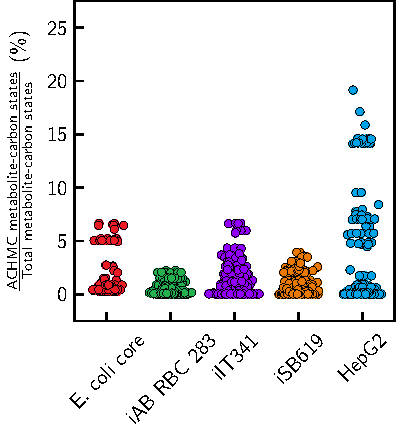
\includegraphics[width=\textwidth]{subpanels/figure-jitter-fraction-mc-states-carbon.pdf}
    \end{subfigure}
    \begin{subfigure}[t]{0.495\textwidth}
        \caption{}
        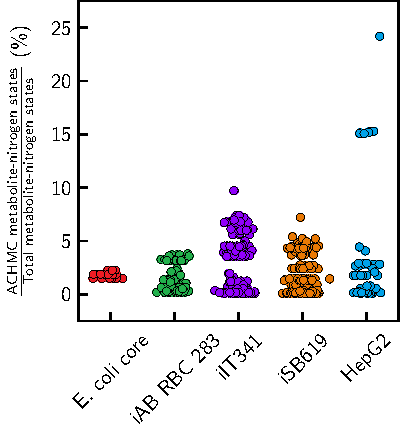
\includegraphics[width=\textwidth]{subpanels/figure-jitter-fraction-mc-states-nitrogen.pdf}
    \end{subfigure}
\end{figure}

\end{document}

